\documentclass[10pt,a4paper, margin=1in]{article}
\usepackage{fullpage}
\usepackage{amsfonts, amsmath, pifont}
\usepackage{amsthm}
\usepackage{graphicx}
\usepackage{float}

\usepackage{tkz-euclide}
\usepackage{tikz}
\usepackage{pgfplots}
\pgfplotsset{compat=1.13}

\usepackage{listings}
\usepackage{color}

% Define colors for syntax highlighting
\definecolor{codegreen}{rgb}{0,0.6,0}
\definecolor{codegray}{rgb}{0.5,0.5,0.5}
\definecolor{codepurple}{rgb}{0.58,0,0.82}
\definecolor{backcolour}{rgb}{0.95,0.95,0.92}

% Setup the style for the Python code
\lstset{language=Python,
        backgroundcolor=\color{backcolour},   
        commentstyle=\color{codegreen},
        keywordstyle=\color{magenta},
        numberstyle=\tiny\color{codegray},
        stringstyle=\color{codepurple},
        basicstyle=\ttfamily\footnotesize,
        breakatwhitespace=false,         
        breaklines=true,                 
        captionpos=b,                    
        keepspaces=true,                 
        numbers=left,                    
        numbersep=5pt,                  
        showspaces=false,                
        showstringspaces=false,
        showtabs=false,                  
        tabsize=2
}

\usepackage{geometry}
 \geometry{
 a4paper,
 total={210mm,297mm},
 left=10mm,
 right=10mm,
 top=10mm,
 bottom=16mm,
 }
 % Write both of your names here. Fill exxxxxxx with your ceng mail address.
 \author{
  Akçan, Batuhan\\
  \texttt{e2580181@ceng.metu.edu.tr}
  \and
  Sönmezer, Mert\\
  \texttt{e2516920@ceng.metu.edu.tr}
}

\title{CENG 384 - Signals and Systems for Computer Engineers \\
Spring 2024 \\
Homework 4}
\begin{document}
\maketitle



\noindent\rule{19cm}{1.2pt}

\begin{enumerate}

\item %write the solution of q1  
    \begin{enumerate}
    % Write your solutions in the following items.
        \item %write the solution of q1a
            \begin{figure}[htbp]
                \centering
                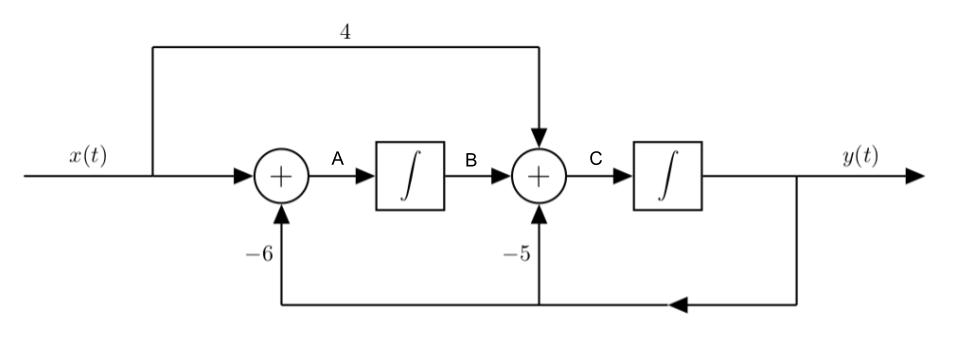
\includegraphics[width=1\linewidth]{q1a.jpg}
                \caption{Question 1 part a}
                \label{fig:q1a}
            \end{figure}\vspace{0.3cm}
            To find the differential equation of the system represented in Figure 1, we need to find the expressions corresponding to each letter.
            \begin{align*}
                A &= x(t) - 6y(t) \\
                B &= \int Adt = \int(x(t) - 6y(t))dt \\
                C &= 4x(t) - 5y(t) + B = 4x(t) - 5y(t) + \int(x(t) - 6y(t))dt \\
                y(t) &= \int Cdt = \int \Bigl( 4x(t) - 5y(t) + \int(x(t) - 6y(t))dt \Bigr) dt
            \end{align*}
            As you see, we obtained $y(t)$, but it is still not in the desired form. Now, let's convert it into the constant coefficient differential equation form.
            \begin{align*}
                y'(t) = 4x(t) - 5y((t) + \int(x(t) - 6y(t))dt \\
                y'(t) + 5y(t) - 4x(t) = \int(x(t) - 6y(t))dt \\
                y''(t) + 5y'(t) - 4x'(t) = x(t) - 6y(t)
            \end{align*}
            After some basic algebraic manipulations applied to the equation above, it can be obtain the following equation:
            $$y''(t) + 5y'(t) + 6y(t) = x(t) + 4x'(t)$$
        \item %write the solution of q1b
        Frequency response of the system can be found by leveraging the linearity property of the Fourier Transform. Firstly, starting with taking the Fourier Transform of both sides will be a reasonable choice.
        $$(j\omega)^2Y(j\omega)+5(j\omega)Y(j\omega)+6Y(j\omega)=X(j\omega)+4(j\omega)X(j\omega)$$
        Then, let us replace the input by an impulse function and its Fourier transform, which is,
        $$x(t)=\delta(t)\rightarrow X(j\omega)=1$$
        Utilizing the equation above, let's try to hit the frequency response of the system defined in the question.
        \begin{align*}
            ((j\omega)^2+5(j\omega)+6)Y(j\omega) = 4(j\omega)+1 \\
            H(j\omega) = \frac{4(j\omega)+1}{(j\omega)^2+5(j\omega)+6}
        \end{align*}
        \item %write the solution of q1c
        Finding the inverse Fourier Transform of the frequency response gives us the impulse response of the system.
        $$ H(j\omega) = \frac{4(j\omega)+1}{(j\omega)^2+5(j\omega)+6} \rightarrow h(t)$$
	To find the inverse Fourier Transform, we can utilize the partial fraction          method.
        \begin{align*}
            \frac{4(j\omega)+1}{(j\omega)^2+5(j\omega)+6} = \frac{A}{2 + j\omega} + \frac{B}{3 + j\omega} \\
            Aj\omega + 3A + Bj\omega + 2B = 4j\omega + 1\\
        \end{align*}
        This gives us the following equations:
        \begin{align*}
            A+B=4\\
            3A+2B=1\\
            A=-7 \text{ and } B=11
        \end{align*}
        Namely,
        $$H(j\omega) = \frac{-7}{2 + j\omega} + \frac{11}{3 + j\omega}$$
        Now, let's calculate the inverse Fourier Transform.
        $$h(t)=(-7e^{-2t}+11e^{-3t})u(t)$$
        \item %write the solution of q1d
        We can use the following formula to get the output of the system:
        $$Y(j\omega) = H(j\omega)X(j\omega)$$
        We first need to find the inverse Fourier Transform of the input $x(t)$.
        $$x(t) = \frac{1}{4}e^{\frac{-t}{4}}u(t) \rightarrow X(j\omega) = \frac{1}{1 + 4j\omega}$$
        When multiplying the $H(j\omega)$ and $X(j\omega)$,
        $$H(j\omega)X(j\omega) = \frac{1+ 4j\omega}{((j\omega)^2+5j\omega+6)} \frac{1}{(1+ 4j\omega)} = \frac{1}{(j\omega)^2+5j\omega+6} = \frac{1}{2 + j\omega} + \frac{1}{3 + j\omega} = Y(j\omega)$$
        Then, finding the inverse Fourier Transform of the expression above hits $y(t)$.
        $$Y(j\omega) = \frac{1}{2 + j\omega} + \frac{1}{3 + j\omega}\rightarrow y(t)=(e^{-2t}+e^{-3t})u(t)$$
    \end{enumerate}

\item %write the solution of q2  
	\begin{enumerate}
    % Write your solutions in the following items.
    \item %write the solution of q2a
    We have\vspace{0.3cm}\\
    $H(jw) = \frac{jw+4}{(jw)^2+5jw+6} = \frac{Y(jw)}{X(jw)}$\vspace{0.3cm}\\
    Hence\vspace{0.3cm}\\
    $jwX(jw) + 4X(jw) = (jw)^2Y(jw)+5jwY(jw)+6Y(jw)$\vspace{0.3cm}\\
    According to tables 4.1 and 4.2, taking the inverse Fourier Transform, we get\vspace{0.3cm}\\
    $\frac{d}{dt}x(t)+4x(t) = \frac{d^2}{dt^2}y(t)+5\frac{d}{dt}y(t)+6y(t)$.\vspace{0.3cm}\\
    \item %write the solution of q2b
    We have\vspace{0.3cm}\\
    $H(jw) = \frac{jw+4}{(jw+3)(jw+2)} = \frac{A}{jw+3}+\frac{B}{jw+2} = \frac{(A+B)jw+2A+3B}{(jw+3)(jw+2)}$\vspace{0.3cm}\\
    We have the equations\vspace{0.3cm}\\
    $A+B=1\;$ and $\; 2A+3B=4$\vspace{0.3cm}\\
    Therefore,\vspace{0.3cm}\\
    $A=-1,\; B=2.$\vspace{0.3cm}\\
    Hence,\vspace{0.3cm}\\
    $H(jw) = \frac{-1}{jw+3}+\frac{2}{jw+2}$.\vspace{0.3cm}\\
    According to tables 4.1 and 4.2, taking the inverse Fourier Transform, we get\vspace{0.3cm}\\
    $h(t) = (-e^{-3t}+2e^{-2t})u(t).$\vspace{0.3cm}\\
	\item %write the solution of q2c
	According to tables 4.1 and 4.2, Fourier Transform of the given $\;x(t)\;$ is\vspace{0.3cm}\\
    $X(jw) = \frac{1}{4+jw} - \frac{1}{(4+jw)^2} = \frac{3+jw}{(4+jw)^2}.$\vspace{0.3cm}\\
    We know that\vspace{0.3cm}\\
    $Y(jw) = X(jw)H(jw) = \frac{jw+4}{(jw+3)(jw+2)}\cdot \frac{3+jw}{(4+jw)^2} = \frac{1}{(jw+2)(jw+4)}.$\vspace{0.3cm}\\
	\item %write the solution of q2d
	We have\vspace{0.3cm}\\
    $Y(jw) = \frac{1}{(jw+2)(jw+4)} = \frac{A}{jw+2} + \frac{B}{jw+4} = \frac{(A+B)jw+4A+2B}{(jw+2)(jw+4)}.$\vspace{0.3cm}\\
    We have the equations\vspace{0.3cm}\\
    $A+B=0\;$ and $\; 4A+2B=1$.\vspace{0.3cm}\\
    Hence, we have\vspace{0.3cm}\\
    $A=\frac{1}{2},\; B=\frac{-1}{2}$\vspace{0.3cm}\\
    Thus, we can write\vspace{0.3cm}\\
    $Y(jw) = \frac{1}{2}\frac{1}{jw+2}-\frac{1}{2}\frac{1}{jw+4}.$\vspace{0.3cm}\\
    According to tables 4.1 and 4.2, taking the inverse Fourier Transform, we get\vspace{0.3cm}\\
    $y(t) = (\frac{1}{2}e^{-2t}-\frac{1}{2}e^{-4t})u(t).$\vspace{0.3cm}\\
    \end{enumerate}

\item %write the solution of q3
    \begin{enumerate}
    % Write your solutions in the following items.
    \item %write the solution of q3a
    Recall the following formula:
    $$Y(e^{j\omega})=H(e^{j\omega})X(e^{j\omega})$$
    The Fourier Transform of the input-output pair should be found separately.
    $$x[n]=\biggl(\frac{2}{3}\biggr)^nu[n] \longleftrightarrow X(e^{j\omega})=\frac{1}{1-\frac{2}{3}e^{-j\omega}}$$
    The expression above represents the Fourier Transform of the input $x[n]$. Now, let's turn to $y[n]$
    $$y[n]=n\biggl( \frac{2}{3}\biggr)^{n+1}u[n] = \frac{2}{3}n\biggl( \frac{2}{3}\biggr)^nu[n] = \frac{2}{3}(n+1-1)\biggl( \frac{2}{3}\biggr)^nu[n] = \frac{2}{3} \Biggl( (n+1)\biggl( \frac{2}{3}\biggr)^nu[n]- \biggl( \frac{2}{3}\biggr)^nu[n]\Biggr)$$
    Now, we can utilize the linearity property of Fourier Transform.
    $$y[n]=n\biggl( \frac{2}{3}\biggr)^{n+1}u[n] \longleftrightarrow Y(e^{j\omega})=\frac{2}{3}\biggl(\frac{1}{(1-\frac{2}{3}e^{-j\omega})^2} - \frac{1}{1-\frac{2}{3}e^{-j\omega}} \biggr)$$
    Now, let's find the frequency response,
    $$H(e^{j\omega})=\frac{Y(e^{j\omega})}{X(e^{j\omega})}=\frac{2}{3}\biggl(\frac{1}{(1-\frac{2}{3}e^{-j\omega})^2} - \frac{1}{1-\frac{2}{3}e^{-j\omega}} \biggr)\biggl( 1-\frac{2}{3}e^{-j\omega}\biggr)$$
    After equating the denominators and some algebraic manipulations, we obtain $H(e^{j\omega})$ as follows:
    $$H(e^{j\omega})=\frac{\frac{4}{9}e^{-j\omega}}{1-\frac{2}{3}e^{-j\omega}}$$
    \item %write the solution of q3b
    To find the impulse response of the system, we need to find the inverse Fourier Transform of the frequency response. Firstly, let's apply the partial fraction method.
    \begin{align*}
        &H(e^{j\omega}) = \frac{\frac{4}{9}e^{-j\omega}}{1-\frac{2}{3}e^{-j\omega}} = \frac{4e^{-j\omega}}{9-6e^{-j\omega}} \\
        &\frac{4e^{-j\omega}}{9-6e^{-j\omega}} = \frac{A}{3} + \frac{B}{3-2e^{-j\omega}}\\
        &3A - 2Ae^{-j\omega}+3B=4e^{-j\omega}\\
        &A=-2 \text{ and } B=2
    \end{align*}
    Then, we get the following equation:
    $$H(e^{j\omega})=\frac{-2}{3} + \biggl(\frac{2}{3}\biggr)\frac{1}{1-\frac{2}{3}e^{-j\omega}}$$
    Now, we can find the inverse Fourier Transform of each term and sum them up.
    $$H(e^{j\omega}) \longleftrightarrow h[n]=\frac{-2}{3}\delta[n]+\biggl(\frac{2}{3}\biggr)^{n+1}u[n]$$
    \item %write the solution of q3c
    We know that
    $$H(e^{jw}) = \frac{Y(e^{jw})}{X(e^{jw})} = \frac{\frac{4}{9}e^{-j\omega}}{1-\frac{2}{3}e^{-j\omega}}$$
    Hence, we get the following equation:
    $$\frac{4}{9}e^{-j\omega}X(e^{j\omega})=Y(e^{j\omega})-\frac{2}{3}e^{-j\omega}Y(e^{j\omega})$$
    When applying the inverse Fourier Transform to the equation above, the difference equation is obtained as follows:
    $$y[n]=\frac{2}{3}y[n-1]+\frac{4}{9}x[n-1]$$
    \item %write the solution of q3d
    Figure 2 illustrates the block diagram of the system.
        \begin{figure}[htbp]
            \centering
            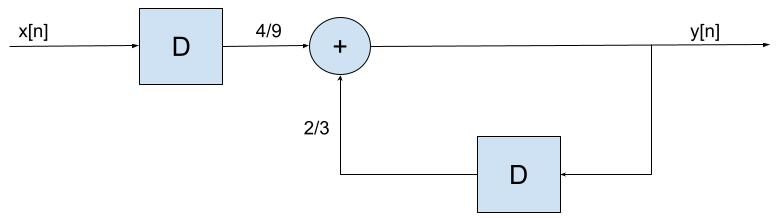
\includegraphics[width=1\linewidth]{q3d.jpg}
            \caption{Question 3 part d}
            \label{fig:q3d}
        \end{figure}\vspace{0.3cm}
    \end{enumerate}

\item %write the solution of q4
	\begin{enumerate}
    % Write your solutions in the following items.
    \item %write the solution of q4a
    We have\vspace{0.3cm}\\
    $2x[n]-\frac{1}{8}y[n-2]+\frac{3}{4}y[n-1]=y[n]$\vspace{0.3cm}\\
    Rearranging the terms, we get\vspace{0.3cm}\\
    $y[n]-\frac{3}{4}y[n-1]+\frac{1}{8}y[n-2] = 2x[n]$.\vspace{0.3cm}\\
    \item %write the solution of q4b
    Taking the Fourier Transform of the difference equation, we get\vspace{0.3cm}\\
    $Y(e^{jw})-\frac{3}{4}e^{-jw}Y(e^{jw})+\frac{1}{8}e^{-2jw}Y(e^{jw}) = 2X(e^{jw})$\vspace{0.3cm}\\
    $H(e^{jw}) = \frac{Y(e^{jw})}{X(e^{jw})} = \frac{2}{1-\frac{3}{4}e^{-jw}+\frac{1}{8}e^{-2jw}}.$\vspace{0.3cm}\\
	\item %write the solution of q4c
	We have\vspace{0.3cm}\\
    $H(e^{jw}) = \frac{2}{(1-\frac{1}{2}e^{-jw})(1-\frac{1}{4}e^{-jw})} = \frac{A}{1-\frac{1}{2}e^{-jw}}+\frac{B}{1-\frac{1}{4}e^{-jw}} = \frac{(\frac{-A}{4}+\frac{-B}{2})e^{-jw}+A+B}{(1-\frac{1}{2}e^{-jw})(1-\frac{1}{4}e^{-jw})}$\vspace{0.3cm}\\
    We get the equations\vspace{0.3cm}\\
    $\frac{-A}{4}+\frac{-B}{2} = 0\;$ and $A+B=2$\vspace{0.3cm}\\
    Hence, we have\vspace{0.3cm}\\
    $A=4,\; B=-2.$\vspace{0.3cm}\\
    So, we get\vspace{0.3cm}\\
    $H(e^{jw}) = \frac{4}{1-\frac{1}{2}e^{-jw}}+\frac{-2}{1-\frac{1}{4}e^{-jw}}.$\vspace{0.3cm}\\
    According to Table 5.2, taking the inverse Fourier Transform, we get\vspace{0.3cm}\\
    $h[n] = (4\cdot (\frac{1}{2})^n -2 \cdot (\frac{1}{4})^n)\cdot u[n]$\vspace{0.3cm}\\
	\item %write the solution of q4d
	According to Table 5.2, Fourier Transform of the input is\vspace{0.3cm}\\
    $X(e^{jw}) = \frac{1}{1-\frac{1}{4}e^{-jw}}$\vspace{0.3cm}\\
    We know that\vspace{0.3cm}\\
    $Y(e^{jw}) = X(e^{jw})H(e^{jw}) = \frac{2}{(1-\frac{1}{2}e^{-jw})(1-\frac{1}{4}e^{-jw})^2} = \frac{A}{1-\frac{1}{2}e^{-jw}} + \frac{Be^{-jw} + C}{(1-\frac{1}{4}e^{-jw})^2} = \frac{(\frac{A}{16}+\frac{-B}{2})e^{-2jw}+(\frac{-A}{2}+B+\frac{-C}{2})e^{-jw}+A+C}{(1-\frac{1}{2}e^{-jw})(1-\frac{1}{4}e^{-jw})^2}$\vspace{0.3cm}\\
    We have the equations\vspace{0.3cm}\\
    $\frac{A}{16}+\frac{-B}{2}=0,\; \frac{-A}{2}+B+\frac{-C}{2}=0,\; A+C=2$\vspace{0.3cm}\\
    Solving the equations, we get\vspace{0.3cm}\\
    $A=8,\; B=1,\; C=-6$\vspace{0.3cm}\\
    Hence, we have\vspace{0.3cm}\\
    $Y(e^{jw}) = \frac{8}{1-\frac{1}{2}e^{-jw}} + \frac{e^{-jw}-6}{(1-\frac{1}{4}e^{-jw})^2} = \frac{8}{1-\frac{1}{2}e^{-jw}} + \frac{e^{-jw}-4}{(1-\frac{1}{4}e^{-jw})^2} + \frac{-2}{(1-\frac{1}{4}e^{-jw})^2} = \frac{8}{1-\frac{1}{2}e^{-jw}} - \frac{4}{1-\frac{1}{4}e^{-jw}} + \frac{-2}{(1-\frac{1}{4}e^{-jw})^2}$\vspace{0.3cm}\\
    Taking the Inverse Fourier Transform, according to the tables 5.1 and 5.2, we get\vspace{0.3cm}\\
    $y[n] = (-4\cdot (\frac{1}{4})^n -2 \cdot (n+1) \cdot (\frac{1}{4})^n + 8 \cdot (\frac{1}{2})^n)\cdot u[n]$\vspace{0.3cm}\\
    \end{enumerate}

\item %write the solution of q5 
As we can see from the block diagram,\vspace{0.3cm}\\
$y[n] = x[n] \ast h_1[n] + x[n] \ast h_2[n]$\vspace{0.3cm}\\
Using Linearity Property, converting to the frequency domain, we get\vspace{0.3cm}\\
$Y(e^{jw}) = X(e^{jw})H_1(e^{jw}) + X(e^{jw})H_2(e^{jw}) = X(e^{jw})H(e^{jw})$\vspace{0.3cm}\\
So, we have\vspace{0.3cm}\\
$H(e^{jw}) = H_1(e^{jw}) + H_2(e^{jw})$\vspace{0.3cm}\\
According to Table 5.2, taking the Fourier Transform of $\; h_1[n], \;$ we get\vspace{0.3cm}\\
$H_1(e^{jw}) = \frac{1}{1-\frac{1}{3}e^{-jw}} = \frac{3}{3-e^{-jw}}$\vspace{0.3cm}\\
We know that\vspace{0.3cm}\\
$H_2(e^{jw}) = H(e^{jw}) - H_1(e^{jw}) = \frac{5e^{-jw}-12}{e^{-2jw}-7e^{-jw}+12} - \frac{3}{3-e^{-jw}} = \frac{5e^{-jw}-12}{(e^{-jw}-4)(e^{-jw}-3)} + \frac{3}{e^{-jw}-3}$\vspace{0.3cm}\\
$= \frac{8e^{-jw}-24}{(e^{-jw}-4)(e^{-jw}-3)} = \frac{8}{e^{-jw}-4} = \frac{-2}{1-\frac{1}{4}e^{-jw}}$\vspace{0.3cm}\\
Taking the Inverse Fourier Transform, by the Table 5.2, we get\vspace{0.3cm}\\
$h_2[n] = -2(\frac{1}{4})^nu[n].$\vspace{0.3cm}\\
    
\item %write the solution of q6
\begin{lstlisting}[language=Python, caption=DTFT]
import numpy as np
import matplotlib.pyplot as plt

# Parameters
n_min = -50
n_max = 50
n = np.arange(n_min, n_max + 1)
x_n = (1/2)**np.abs(n)

omega = np.linspace(-3*np.pi, 3*np.pi, 400)
X_omega = np.zeros(len(omega), dtype=complex)

for i, w in enumerate(omega):
    X_omega[i] = np.sum(x_n * np.exp(-1j * w * n))

plt.plot(omega, np.abs(X_omega))
plt.grid(True)
plt.show()
\end{lstlisting}


\end{enumerate}


\end{document}

